% Pacotes e configurações padrão do estilo ``article''\
% -------------------------------------
\documentclass[a4paper,11pt]{article}
% Layout
% --------------------------------------------------------------------------------
%     Gráficos e layout ----------------------------------------------------------------------

\ifx\pdfmatch\undefined
\else
    \usepackage[T1]{fontenc}
    \usepackage[utf8]{inputenc}
\fi
% xetex:
\ifx\XeTeXinterchartoks\undefined
\else
    \usepackage{fontspec}
    \defaultfontfeatures{Ligatures=TeX}
\fi
% luatex:
\ifx\directlua\undefined
\else
    \usepackage{fontspec}
\fi
% End engine-specific settings

%      Fonte --------------------------------------------------------------------------------
%\usepackage{lmodern}
\usepackage{times}
%     Pacotes adicionados -------------------------------------------------------------------
\usepackage{ae}
%     Língua e hifenização ------------------------------------------------------------------
\usepackage[portuguese]{babel}
\usepackage{hyphenat}
%      Outros --------------------------------------------------------------------------------
\usepackage{hyperref} % Permite Links personalisados usando hyperref
\usepackage{fancyhdr}
\usepackage{sectsty}
\usepackage{float}   % Gerencia melhor o posicionamento das figuras e tabelas
%\usepackage{graphicx}
\usepackage[pdftex]{color,graphicx}
\usepackage{hyperref}
\usepackage{enumerate} % Permite alterar Layout do enumerate
%\usepackage{pdflscape}  % Permite alterar a orientação da pagina para Paisagem
%\usepackage{ifthen}  % Permite usar condicionais ifelse
%\usepackage[table]{xcolor} % Permite alterar as cores das células de uma tabela
\usepackage{amsmath,amssymb} % Ambiente para uso de elementos matemáticos
\usepackage{caption}
\usepackage{subcaption} % permite o uso de multiplas figuras com legenda (ambiente subfigure)
\usepackage{minted} % Ambiente minted para colorir código de programas
\usepackage{natbib} % Para referencia bibliográfica
\usepackage{url}    % Referência de links na internet
%\usepackage{listings} % pacote para apresentar código de programação
\usepackage{indentfirst}  % Para indentar o primeiro parágrafo de cada seção
\usepackage{titling}  % Permite Montar uma página de titulo própria

% Layout do documento ------------------------------------------------------------------------
%     Bordas e tamanho da página ------------------------------------------------------------
\usepackage{geometry} 
 \geometry{ % Padrõa ABNT para relatórios
 a4paper,
 left=30mm,
 right=20mm,
 top=30mm,
 bottom=20mm
 }
%     Cabeçalho e Rodapé ---------------------------------------------------------------
\pagestyle{fancy}
  \lhead{}
  \chead{}
  \rhead{}
  \lfoot{}
  \cfoot{}
  \rfoot{\thepage}
%     Númeração ------------------------------------------------------------------------
  \pagenumbering{arabic}
%     Retas do cabeçalho e rodapé ------------------------------------------------------
  \renewcommand{\headrulewidth}{0.5pt}
  \renewcommand{\footrulewidth}{0.5pt}
%     Tamanho da letra de seções e derivadas --------------------------------------------
  \sectionfont{\normalsize}
  \subsectionfont{\small}
%     Hiperlinks ------------------------------------------------------------------------
  \hypersetup{
                  colorlinks,
                  citecolor=black,
                  filecolor=black,
                  linkcolor=black,
                  urlcolor=black
                  }
%     Definições do pdf ----------------------------------------------------------------------
\hypersetup{
    unicode=false,          % non-Latin characters in Acrobat’s bookmarks
    pdftoolbar=true,        % show Acrobat’s toolbar?
    pdfmenubar=true,        % show Acrobat’s menu?
    pdffitwindow=false,     % window fit to page when opened
    pdfstartview={FitH},    % fits the width of the page to the window    
    pdfauthor={Rafael Lima},     % author
    pdfnewwindow=true      % links in new window
}
%     Outros ----------------------------------------------------------------------------
      %\renewcommand{\thesection}{(\alph{section})} % muda o estilo de númeração das sections
      % alterando a formatação dos numeradores de lista de itens
      \renewcommand\theenumi{\arabic{enumi}}
      \renewcommand\labelenumi{(\textit{\theenumi})}
	  \renewcommand\theenumii{\arabic{enumii}}
	  \renewcommand\labelenumii{(\textit{\theenumi.\theenumii})}
      
% ---------------------------------------------------------------------------------------


\title{Laboratório X} % Define o título do Relatório
\author{Rafael Lima}

% Definições Auxiliares ( Macros próprias )
% -----------------------------------------------------------------
%\input{relat_aux.tex} % Arquivo com minhas macros
% ----------------------------------~>ø<~---------------------------------------
\begin{document}
% Capa e Índice ---------------------------------------------------------------
%--------------------------------------------------- Capa --------------------------------------------
%\newpage
\begin{figure}[h!]
\centering

\includegraphics[scale=0.9]{img/simb_unb.png}
\label{fig:unb}
\end{figure}

\begin{center}
{\LARGE Universidade de Brasília}\\
Departamento de Engenharia Elétrica (ENE)\\
Professor: Geovany A. Borges\\
Disciplina: Laboratório de Controle Dinâmico\\
\end{center}


\vspace{0.18\textheight}

\begin{center}
    \Huge \textbf{\\\thetitle \\}
\end{center}

\vspace*{\fill} % Completa espaço em branco e empurra o resto para o final da página

% Tabela com os nome das pessoas do grupo

\begin{table}[H]
    \begin{tabular}{ll}
        % Nome      & Matrícula
        Tiago Pereira Neves & 16/0077907 \\
%        Jefferson C. T. O. Lima & 18/0137107 \\
        Rafael Lima & 10/0131093 \\
    \end{tabular}
\end{table}

\vspace{0.5cm}

\begin{center}
    \textbf{Brasília\\
    \the\year} % Coloca o Ano atual
\end{center}

\thispagestyle{empty} % Retira o cabeçalho e o rodapé da página

% ------------------------------------------------- Índice -------------------------------------------
\newpage
\tableofcontents
\newpage
% ----------------------------------------------------------------------------------------------------

 % Capa para UnB
% Conteúdo -------------------------------------------------------------------

% Material de referência - prof
% https://drive.google.com/drive/folders/1IDdc7QVsdYIASgZzNlUelhGF_FaV2_EJ

\section{Descrição da Planta}

\subsection{Modelo Motor DC}

% Como modelar um motor ------------------------------
% http://ctms.engin.umich.edu/CTMS/index.php?example=MotorSpeed&section=SystemModeling
% http://ctms.engin.umich.edu/CTMS/index.php?example=MotorSpeed&section=SimulinkModeling
% http://www.inf.fu-berlin.de/lehre/WS04/Robotik/motors.pdf
% https://ir.nctu.edu.tw/bitstream/11536/125183/36/509-2.pdf
% http://users.isr.ist.utl.pt/~alex/micd0506/motordc.pdf
% http://homepages.laas.fr/lzaccari/seminars/DCmotors.pdf
% https://www.control.isy.liu.se/student/tsrt21/file/pm_dcmotor.pdf

% Técnica antiga de controle ------------------------
% https://en.wikipedia.org/wiki/Ward_Leonard_control

\section{Identificação de Parâmetros}

% http://www.eletrica.ufpr.br/~gustavo/controle_digital/Intro_Ident_Intro_v23abr12.pdf
% convert from ft to ss https://www.mathworks.com/help/signal/ref/tf2ss.html
% convert from ss to ft https://www.mathworks.com/help/matlab/ref/ss2tf.html

Para validar o sistema foi definido um planta para simular o comportamento de um sistema de primeira ordem e um sistema de segunda ordem para uma mesma entrada. O sinal de entrada e a resposta de saída do sistema é então armazenado em arquivo \textit{.mat} para leitura posterior.

% Modelo Figura
\begin{figure}[H]
    \centering
    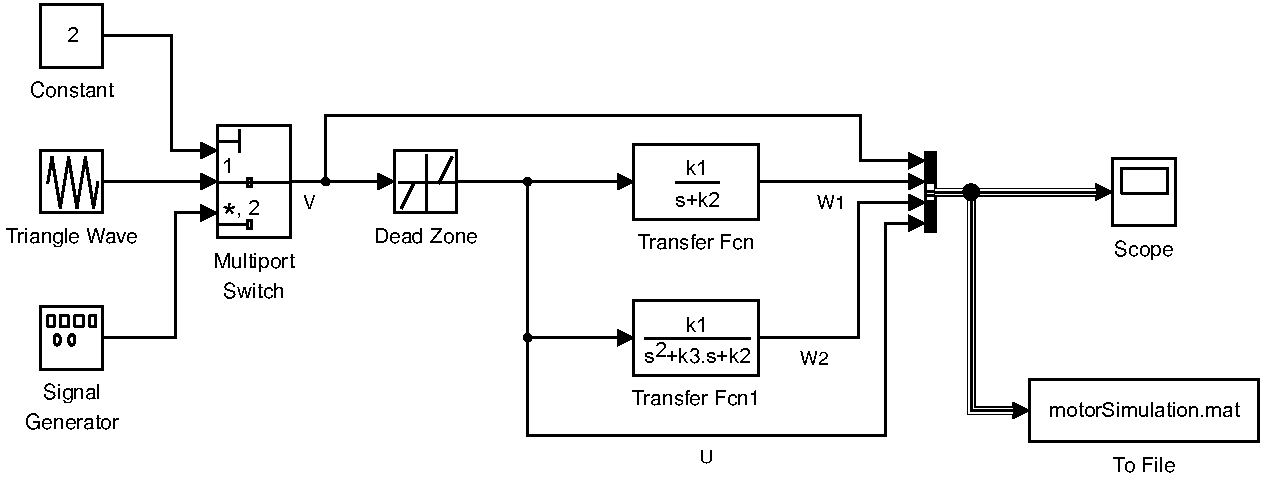
\includegraphics[width=1.0\linewidth]{tex/img/dcMotorSimulation.pdf}
    \caption{Planta Simulação}
    \label{fig:my_label}
\end{figure}

\subsection{Região não Linear - Zona Morta}

% Maior valor da entrada pelo qual a saída é zero.

% Colocar Valores obtidos pelo matlab

\subsection{Estimação modelo como primeira ordem}

Supondo um modelo de primeira ordem com coeficientes $k_1$ e $k_2$ definido por:

\begin{equation}
    H_1(s) = \frac{Y(s)}{X(s)} = \frac{1}{k_1 s+ k_2}
\end{equation}

% Equação de Transferência

Podemos reescrever a função de transferência como
\begin{equation}
k_1 Ys + k_2 Y  = X
\end{equation}

% EDO
A partir do qual temos o sistema descrito a partir da seguinte equação diferencial:

\begin{equation}
k_1 \dot{y}(t) + k_2 y(t) = x(t)
\end{equation}

Tomando os valores de entrada e saída do sistema em diferentes instantes para um sinal de entrada temos:

% Sistema Linear
\begin{equation}
\left\{\begin{array}{c}
    k_1 \dot{y}(t_0) + k_2 y(t_0) = x(t_0)  \\
    \dots\\
    k_1 \dot{y}(t_i) + k_2 y(t_i) = x(t_i)  \\
\end{array} \right.
\end{equation}

% Representação como Matriz

Podemos representar a equação na forma matricial:

\begin{equation}
\left[\begin{array}{cc}
    \dot{y}(t_0) & y(t_0)\\
    \dots  & \dots \\
    \dot{y}(t_i) & y(t_i)\\
\end{array} \right]
\left[\begin{array}{c}
    k_1\\
    k_2\\
\end{array} \right]
=
\left[\begin{array}{c}
    x(t_0)  \\
    \dots\\
    x(t_i)  \\
\end{array} \right]
\end{equation}

% Resolução por Matrizes

Denominando $A$ a matriz envolvendo $\dot{y}(t)$ e $y(t)$, $Bt)$ a matriz dos valores de entrada $x(t)$

\begin{equation}
    A(t) P = B(t)
\end{equation}

\begin{equation}
    A^T(t)A(t) P = A^T(t) B(t)
\end{equation}

Isolando a matriz $P$ podemos achar o parâmetros a partir da seguinte expressão:

\begin{equation}
    P = \left(A^T(t) A(t)\right)^{-1} A^T(t) B(t)
\end{equation}

Para implementar em MATLAB podemos aproximar $\dot{y}(t)$ pelo método de diferenças finitas como

\begin{equation}
\dot{y}(t_i) = \dot{y}[t_i] = \frac{y[t_i] - y[t_{i-1}]}{t_i - t_{i-1}}
\end{equation}

Usando operações de matrizes o código fica bem compacto, como mostrado abaixo:

% Código
\inputminted[frame=single,framesep=10pt]{matlab}{../src/matlab/firstordertf.m}

\subsection{Modelo Linear 2 ordem}

Supondo um modelo de primeira ordem com coeficientes $k_1$, $k_2$ e $k_3$ definido por:

\begin{equation}
    H_2(s) = \frac{Y(s)}{X(s)} = \frac{1}{k_1 s^2+ k_2 s+ k_3}
\end{equation}

% Equação de Transferência

Podemos reescrever a função de transferência como
\begin{equation}
k_1 Ys^2 + k_2 Ys + k_3 Y  = X
\end{equation}

% EDO
A partir do qual temos o sistema descrito a partir da seguinte equação diferencial:

\begin{equation}
k_1 \ddot{y}(t) + k_2 \dot{y}(t) + k_3 y(t) = x(t)
\end{equation}

Tomando os valores de entrada e saída do sistema em diferentes instantes para um sinal de entrada temos:

% Sistema Linear
\begin{equation}
\left\{\begin{array}{c}
    k_1 \ddot{y}(t_0) + k_2 \dot{y}(t_0) + k_3 y(t_0) = x(t_0)  \\
    \dots\\
    k_1 \ddot{y}(t_i) + k_2 \dot{y}(t_i) + k_3 y(t_i) = x(t_i)  \\
\end{array} \right.
\end{equation}

% Representação como Matriz

Podemos representar a equação na forma matricial:

\begin{equation}
\left[\begin{array}{ccc}
    \ddot{y}(t_0) & \dot{y}(t_0) & y(t_0)\\
    \dots  & \dots & \dots \\
    \ddot{y}(t_i) & \dot{y}(t_i) & y(t_i)\\
\end{array} \right]
\left[\begin{array}{c}
    k_1\\
    k_2\\
    k_3\\
\end{array} \right]
=
\left[\begin{array}{c}
    x(t_0)  \\
    \dots\\
    x(t_i)  \\
\end{array} \right]
\end{equation}

% Resolução por Matrizes

De forma similar ao caso de primeira ordem, denominando $A$ a matriz envolvendo $\ddot{y}(t)$, $\dot{y}(t)$ e $y(t)$, $Bt)$ a matriz dos valores de entrada $x(t)$

\begin{equation}
    A(t) P = B(t)
\end{equation}

\begin{equation}
    A^T(t)A(t) P = A^T(t) B(t)
\end{equation}

Isolando a matriz $P$ podemos achar o parâmetros a partir da seguinte expressão:

\begin{equation}
    P = \left(A^T(t) A(t)\right)^{-1} A^T(t) B(t)
\end{equation}

Em MATLAB, usando operações de matrizes a implementação fica bem compacta, como mostrado abaixo:

% Código
\inputminted[frame=single,framesep=10pt]{matlab}{../src/matlab/secondordertf.m}

\subsection{Validação do Método em Simulação}

Aplicando um sinal de entrada em uma planta simulada de primeira ordem com coeficientes escolhidos de forma aleatória, obtemos a seguinte as seguintes respostas para o modelo aproximado de primeira ordem e de segunda ordem, conforme mostrado na figura \ref{fig:model1Evaluation}.

% Modelo Figura
\begin{figure}[H]
    \centering
    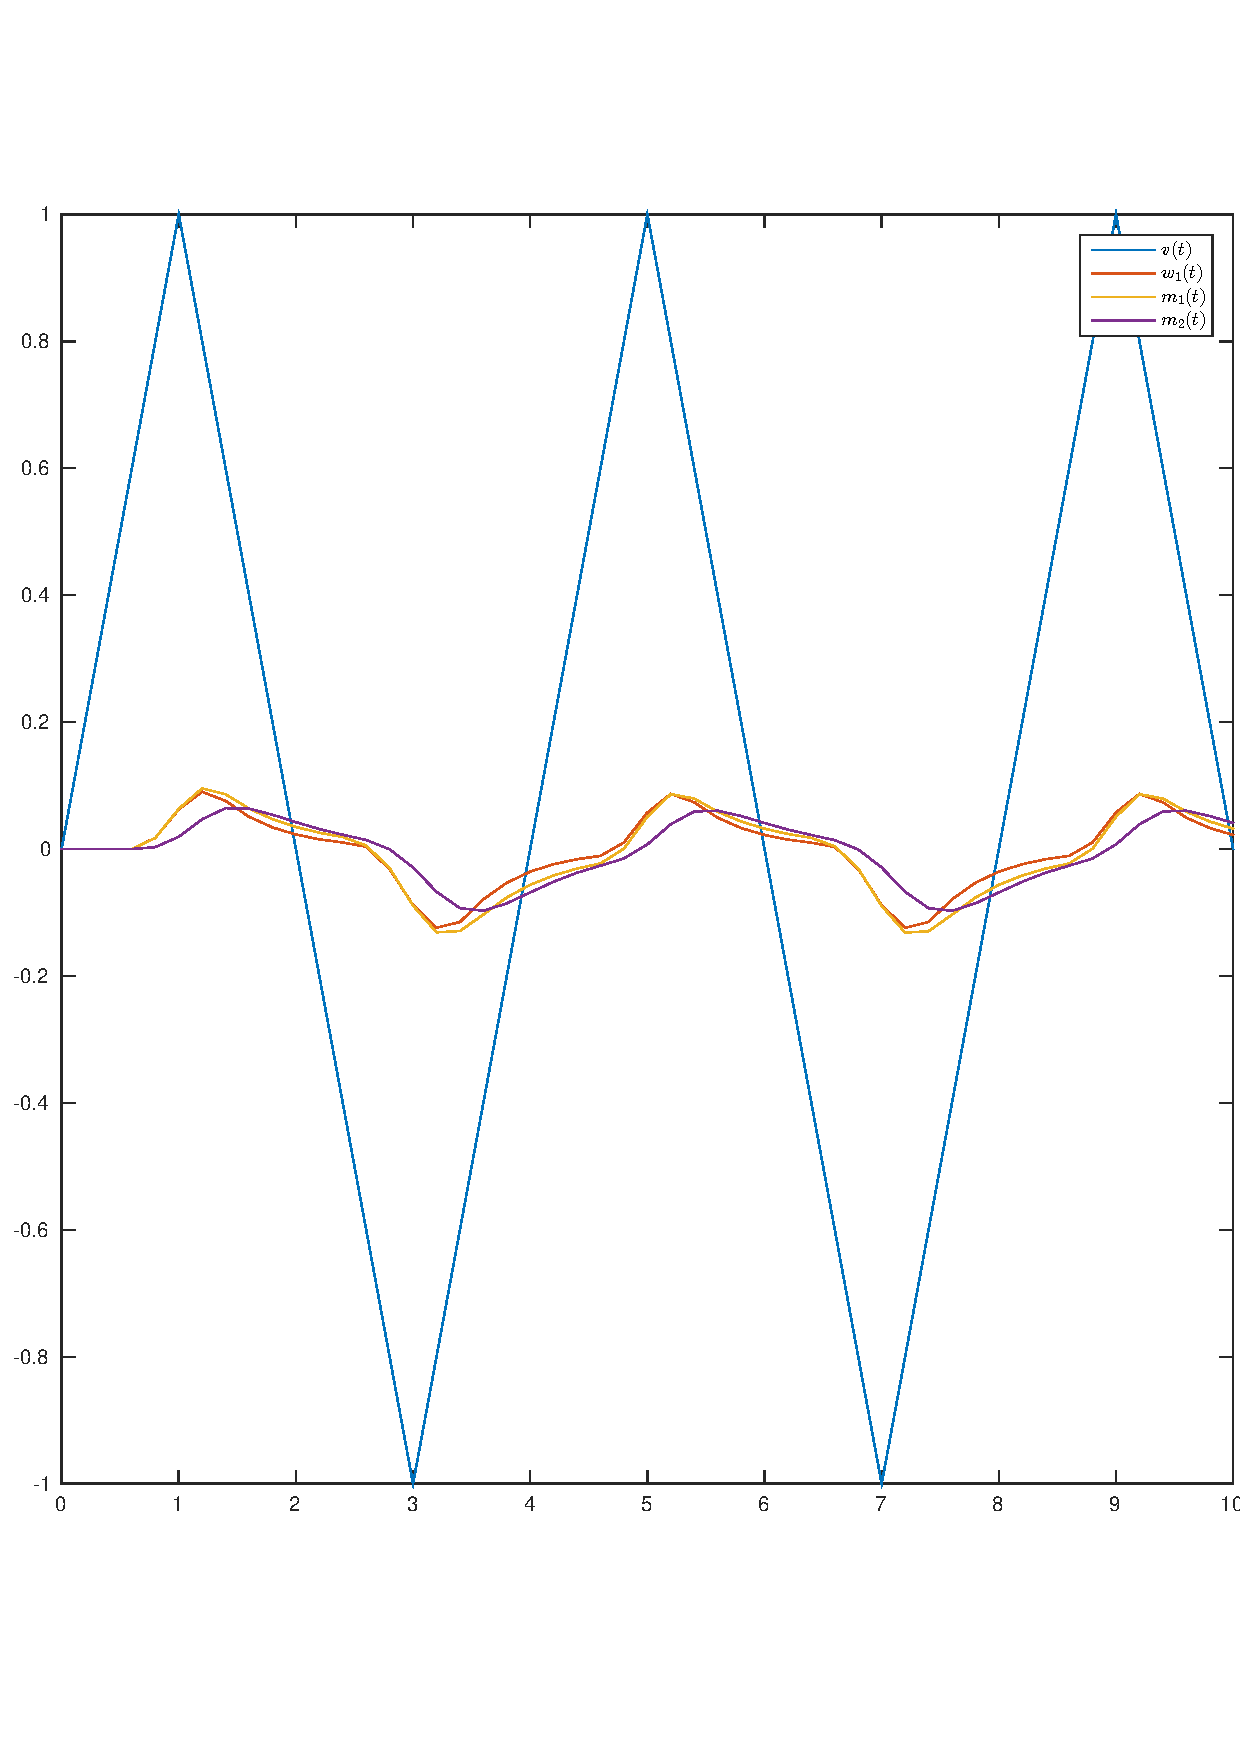
\includegraphics[width=0.6\linewidth]{tex/img/model1Evaluation.pdf}
    \caption{Comparação Modelo Primeira Ordem}
    \label{fig:model1Evaluation}
\end{figure}

Procedendo da mesma forma, aplicando um sinal de entrada em uma planta simulada de segunda ordem com coeficientes escolhidos de forma aleatória, obtemos a seguinte as seguintes respostas para o modelo aproximado de primeira ordem e de segunda ordem, conforme mostrado na figura \ref{fig:model2Evaluation}.

% Modelo Figura
\begin{figure}[H]
    \centering
    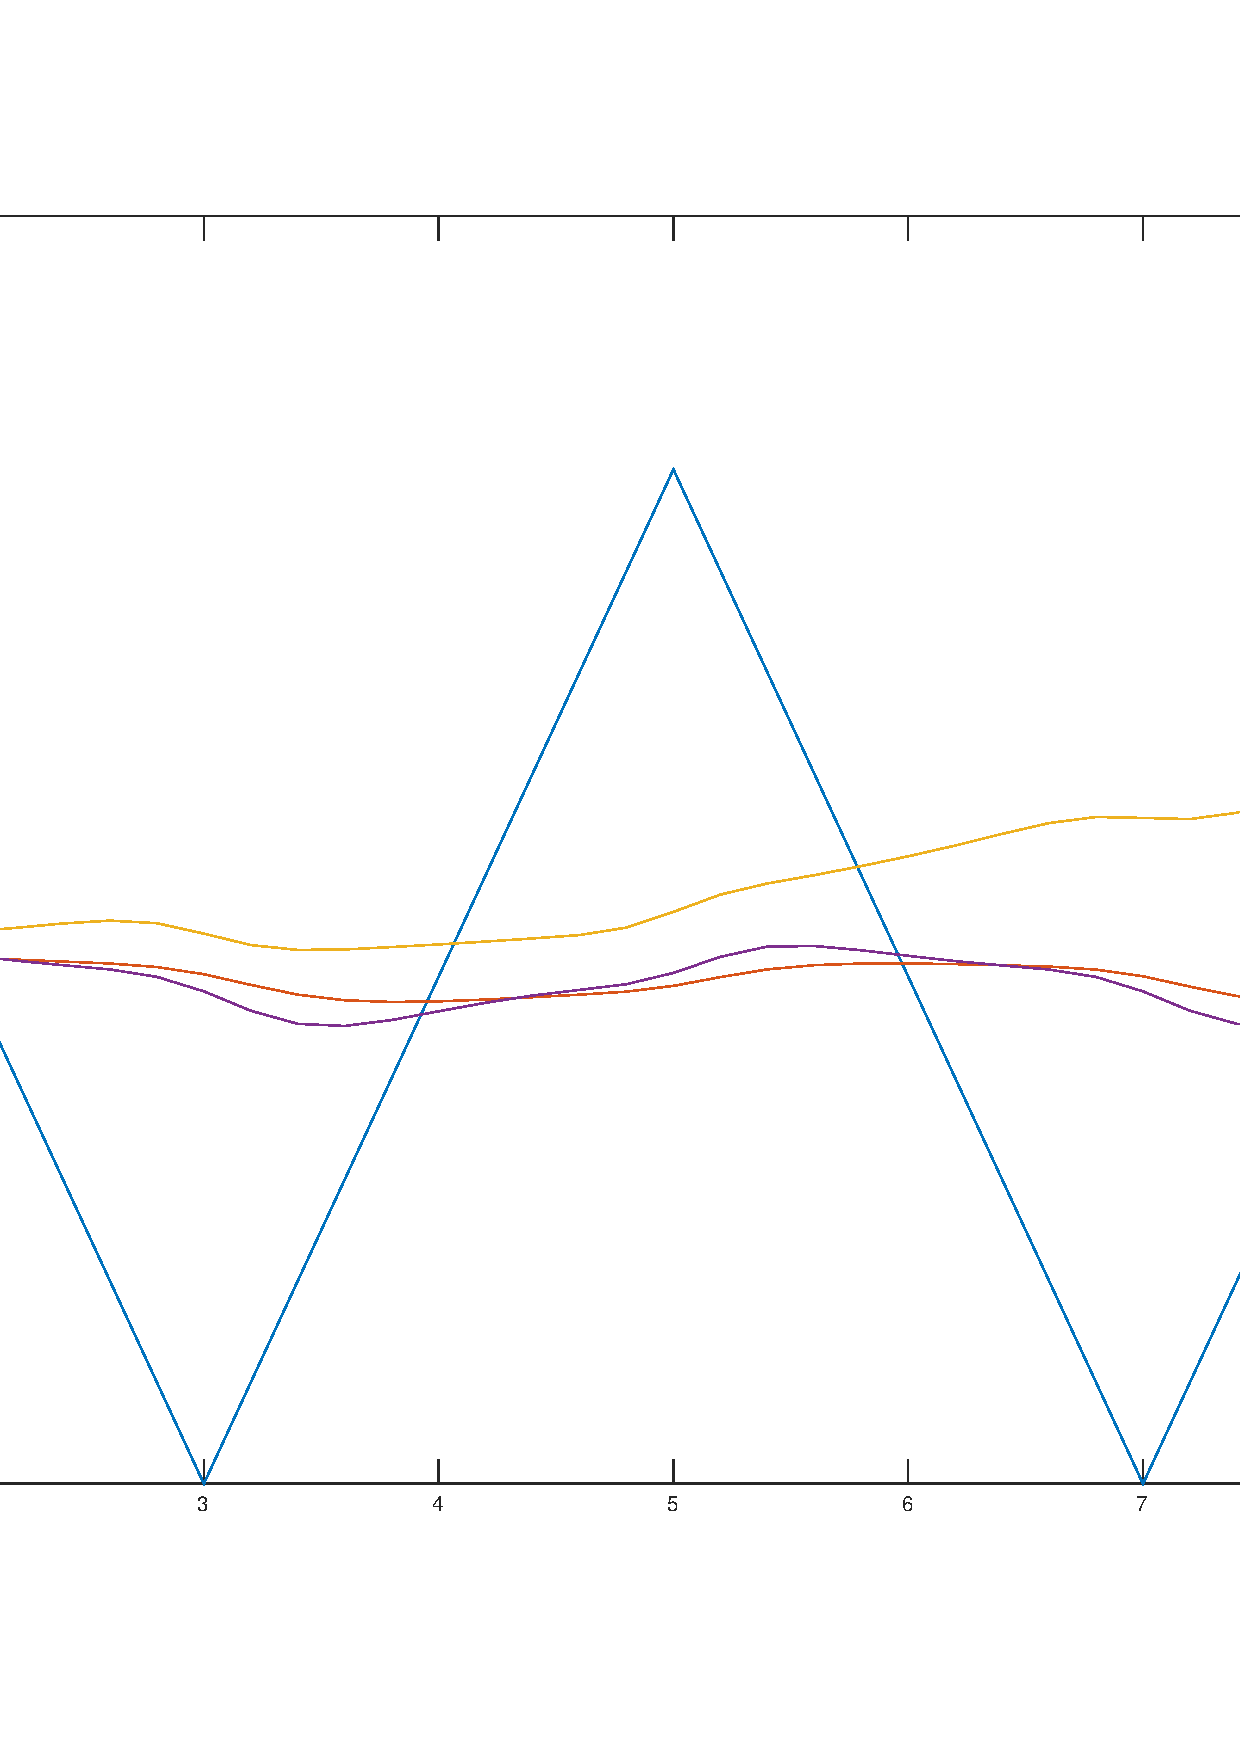
\includegraphics[width=0.6\linewidth]{tex/img/model2Evaluation.pdf}
    \caption{Comparação Modelo Segunda Ordem}
    \label{fig:model2Evaluation}
\end{figure}

Nota-se que em ambos casos, existe um erro entre a resposta do sistema com os parâmetros identificados e o planta original simulada. Isto se deve ao fato que o método de diferenças finitas apenas representa uma aproximação e portanto não representa derivada de forma exata.

Em uma planta real pode ser utilizado algum sensor para medir a velocidade e a aceleração ou ainda adotar alguma aproximação melhor para aproximação da derivada.



% Descrição da Planta
%% Diagrama de descrição


% ---------------------------------------------------------------------------------------

\section{Controle PID}

% Comentar brevemente sobre a estrutura de PID usada
% Anti Windup

\subsection{Planta Simulação PID}

A partir dos dados da identificação, a resposta da planta com o controle PID implementado é simuladas utilizando o Simulink, ilustrada na figura \ref{fig:pidControlPlant}. Na simulação é comparado a resposta ao PID a partir das função de transferência de primeira e de segunda ordem geradas pela etapa de identificação.

\begin{figure}[H]
    \centering
    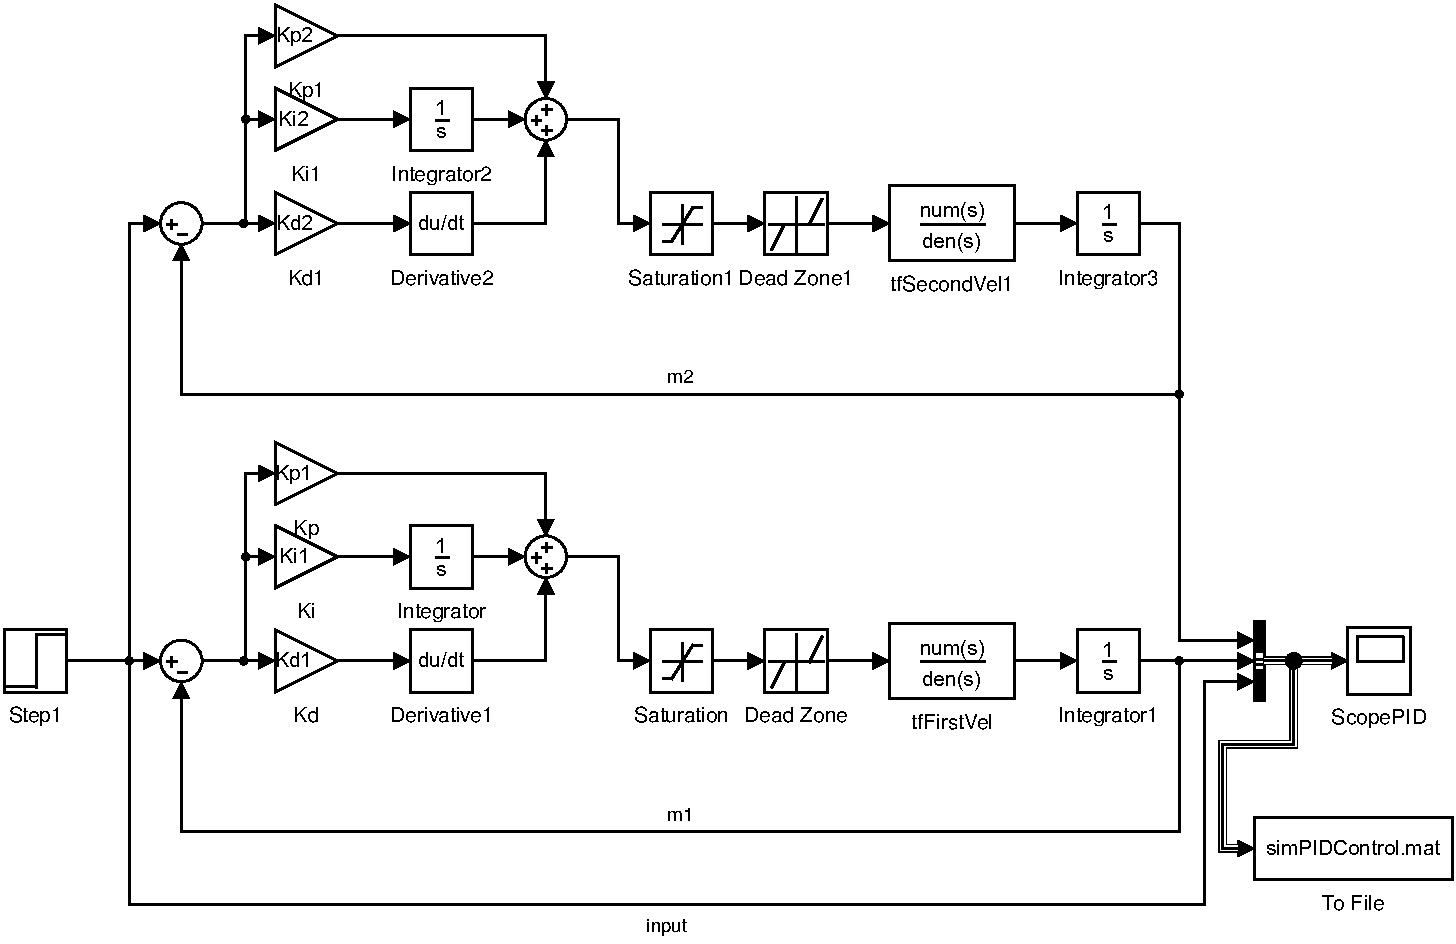
\includegraphics[width=1.0\linewidth]{tex/img/dcMotorControl.pdf}
    \caption{Planta Simulação Controle PID}
    \label{fig:pidControlPlant}
\end{figure}

\subsection{Ajuste dos Parâmetros}

\subsubsection{SISO Tool}

% ---------------------------------------------------------------------------------------

\section{Controle por Espaço de Estados}
\subsection{Modelo em Espaço de Estados}
Como o modelo foi identificado a partir de uma função de transferência é necessário converte para a representação em espaço de estados.

\subsection{Controle por alocação de polos}
A representação por espaço de estados traz a vantagem de permitir posicionar os polos em malha fechada de maneira arbitrária facilitando atender qualquer critério de projeto.

% ---------------------------------------------------------------------------------------
\section{Conclusão}

% ---------------------------------------------------------------------------------------

\bibliographystyle{abbrv}
\bibliography{references}
% Referências
% Acrescentadas no arquivo references.bib
% para usa-las no texto basta usar \citep{}

% ---------------------------------------------------------------------------------------


\end{document}
